\documentclass[aspectratio=169, xcolor={usenames, dvipsnames}]{beamer}
\usetheme[titleformat=plain, % supported values: plain
          logo=i12en,        % supported values: i12en (default), i12de
          itemsize=20pt,
          % defaultitemsep=0.4\baselineskip,
         ]{itc}

% Encoding and language
\usepackage[utf8]{inputenc}
\usepackage[T1]{fontenc}
\usepackage[english]{babel}
\usepackage{listings, listings-rust}
\usepackage{tikz}
\usetikzlibrary{decorations.pathreplacing, arrows}
\usepackage{smartdiagram}
\usesmartdiagramlibrary{additions}
\usepackage[dvipsnames]{xcolor}
\usepackage{fontspec}
\setmainfont{Helvetica}
\setsansfont{Helvetica}
\newfontfamily\DejaSans{DejaVu Sans}
\usepackage{fontawesome}

\makeatletter
\let\old@lstKV@SwitchCases\lstKV@SwitchCases
\def\lstKV@SwitchCases#1#2#3{}
\makeatother
\usepackage{lstlinebgrd}
\makeatletter
\let\lstKV@SwitchCases\old@lstKV@SwitchCases

\lst@Key{numbers}{none}{%
    \def\lst@PlaceNumber{\lst@linebgrd}%
    \lstKV@SwitchCases{#1}%
    {none:\\%
     left:\def\lst@PlaceNumber{\llap{\normalfont
                \lst@numberstyle{\thelstnumber}\kern\lst@numbersep}\lst@linebgrd}\\%
     right:\def\lst@PlaceNumber{\rlap{\normalfont
                \kern\linewidth \kern\lst@numbersep
                \lst@numberstyle{\thelstnumber}}\lst@linebgrd}%
    }{\PackageError{Listings}{Numbers #1 unknown}\@ehc}}
\makeatother

\makeatletter
%%%%%%%%%%%%%%%%%%%%%%%%%%%%%%%%%%%%%%%%%%%%%%%%%%%%%%%%%%%%%%%%%%%%%%%%%%%%%%
%
% \btIfInRange{number}{range list}{TRUE}{FALSE}
%
% Test in int number <number> is element of a (comma separated) list of ranges
% (such as: {1,3-5,7,10-12,14}) and processes <TRUE> or <FALSE> respectively

\newcount\bt@rangea
\newcount\bt@rangeb

\newcommand\btIfInRange[2]{%
    \global\let\bt@inrange\@secondoftwo%
    \edef\bt@rangelist{#2}%
    \foreach \range in \bt@rangelist {%
        \afterassignment\bt@getrangeb%
        \bt@rangea=0\range\relax%
        \pgfmathtruncatemacro\result{ ( #1 >= \bt@rangea) && (#1 <= \bt@rangeb) }%
        \ifnum\result=1\relax%
            \breakforeach%
            \global\let\bt@inrange\@firstoftwo%
        \fi%
    }%
    \bt@inrange%
}
\newcommand\bt@getrangeb{%
    \@ifnextchar\relax%
        {\bt@rangeb=\bt@rangea}%
        {\@getrangeb}%
}
\def\@getrangeb-#1\relax{%
    \ifx\relax#1\relax%
        \bt@rangeb=100000%   \maxdimen is too large for pgfmath
    \else%
        \bt@rangeb=#1\relax%
    \fi%
}

%%%%%%%%%%%%%%%%%%%%%%%%%%%%%%%%%%%%%%%%%%%%%%%%%%%%%%%%%%%%%%%%%%%%%%%%%%%%%%
%
% \btLstHL<overlay spec>{range list}
%
% TODO BUG: \btLstHL commands can not yet be accumulated if more than one overlay spec match.
%
\newcommand<>{\btLstHL}[1]{%
  \only#2{\btIfInRange{\value{lstnumber}}{#1}{\color{orange!30}\def\lst@linebgrdcmd{\color@block}}{\def\lst@linebgrdcmd####1####2####3{}}}%
}%
\makeatother

% Meta information
\title{Visualization of Data Movements and Accesses}
\author{Til Mohr}
% Optional, appears on title page
\presenter{Til Mohr}
\institute{IT Center}
\date{September 25\textsuperscript{th} \& 26\textsuperscript{th}, 2023}

\begin{document}

\lstdefinestyle{mycstyle}{
	language=Rust,
	breaklines=true,
	showstringspaces=false,
	keywordstyle=\color{blue},
	commentstyle=\color{green!50!black},
	%escapeinside=||,
	basicstyle=\ttfamily,
	morecomment=[l][{\color{red!50!black}}]{\#},
	backgroundcolor=\color{black!4},
	numbers=left,
	numbersep=10pt,
	numberstyle=\footnotesize,
	framexleftmargin=0.1cm,
	xrightmargin=0.75cm,
	xleftmargin=0.75cm,
	frame=lines,
	tabsize=4,
	belowskip=0cm,
}


\begin{frame}[plain]
\titlepage
\end{frame}

\begin{frame}[fragile]{Sum of Matrix Elements}
\begin{columns}[T] % align columns
\begin{column}{.48\textwidth}
\setcounter{lstlisting}{0}
\begin{lstlisting}[style=mycstyle, caption={Matrix Summation}, escapechar=!]
let matrix = Matrix::random(2, 2);
let mut sum = 0;
for !{\color{ForestGreen} column}! in !{\color{ForestGreen} 0..2}! {
  for !{\color{red} row}! in !{\color{red} 0..2}! {
    sum += matrix.get(!{\color{red} row}!, !{\color{ForestGreen} column}!);
  }
}
sum
\end{lstlisting}
\hfill
\end{column}%
\hfill%
\begin{column}{.48\textwidth}
\begin{tikzpicture}[
	box/.style={rectangle,draw=black,thick, minimum size=1cm},
]
	\draw[step=1cm,color=gray] (0,0) grid (2,2);
	\node[box,fill=CornflowerBlue] at (0.5,0.5) {3};
	\node[box,fill=CornflowerBlue] at (1.5,0.5) {4};
	\node[box,fill=Goldenrod] at (0.5,1.5) {1};
	\node[box,fill=Goldenrod] at (1.5,1.5) {2};
	\node at (-0.5,1.5) {\color{red} 0};
	\node at (-0.5,0.5) {\color{red} 1};
	\node at (0.5,2.5) {\color{ForestGreen} 0};
	\node at (1.5,2.5) {\color{ForestGreen} 1};
	\node[below right] at (-0.5,4) {Matrix:};

	\only<2->{
		\draw[step=1cm,color=gray] (5,1) grid (4+5,2);
		\node[box,fill=Goldenrod] at (5.5,1.5) {1};
		\node[box,fill=Goldenrod] at (6.5,1.5) {2};
		\node[box,fill=CornflowerBlue] at (7.5,1.5) {3};
		\node[box,fill=CornflowerBlue] at (8.5,1.5) {4};
		\draw[color=gray,line width=3pt] (5,1) rectangle (2+5,2);
		\draw[color=gray,line width=3pt] (2+5,1) rectangle (4+5,2);
		\node[below right] at (-0.5+5,4) {Matrix in Memory:};

		\only<3-4>{
			% Element (0,0)
			\draw[color=black,line width=4pt] (0,1) rectangle (1,2);
			\draw[color=black,line width=4pt] (5,1) rectangle (6,2);
		}
		\only<5-6>{
			% Element (1,0)
			\draw[color=black,line width=4pt] (0,0) rectangle (1,1);
			\draw[color=black,line width=4pt] (7,1) rectangle (8,2);
		}
		\only<7-8>{
			% Element (0,1)
			\draw[color=black,line width=4pt] (1,1) rectangle (2,2);
			\draw[color=black,line width=4pt] (6,1) rectangle (7,2);
		}
		\only<9-10>{
			% Element (1,1)
			\draw[color=black,line width=4pt] (1,0) rectangle (2,1);
			\draw[color=black,line width=4pt] (8,1) rectangle (9,2);
		}
	}

	\only<3->{
		\draw[step=1cm,color=gray] (0,2-5) grid (2,3-5);
		\node[below right] at (-0.5,4.25-5) {Current Item:};
		\only<3-4>{
			\node at (0.5,2.5-5) {\color{red} 0};
			\node at (1.5,2.5-5) {\color{ForestGreen} 0};
		}
		\only<5-6>{
			\node at (0.5,2.5-5) {\color{red} 1};
			\node at (1.5,2.5-5) {\color{ForestGreen} 0};
		}
		\only<7-8>{
			\node at (0.5,2.5-5) {\color{red} 0};
			\node at (1.5,2.5-5) {\color{ForestGreen} 1};
		}
		\only<9-10>{
			\node at (0.5,2.5-5) {\color{red} 1};
			\node at (1.5,2.5-5) {\color{ForestGreen} 1};
		}

		\draw[step=1cm,color=gray] (0+5,2-5) grid (2+5,3-5);
		\node[below right] at (-0.5+5,4.25-5) {Cache:};

		\only<4-5>{
			% Line [(0,0), (0,1)] in cache
			\node[box,fill=Goldenrod] at (0.5+5,2.5-5) {1};
			\node[box,fill=Goldenrod] at (1.5+5,2.5-5) {2};

			\only<4>{
				\draw[decorate,decoration={brace,amplitude=8pt,mirror,raise=4ex}] (5,2) -- (7,2) node[midway] {};
				\draw[->,line width=1pt] (6,0.4) to [out=270,in=30] (7,-2);
				\draw[color=black,line width=4pt] (0+5,2-5) rectangle (1+5,3-5);
			}
		}

		\only<6-7>{
			% Line [(1,0), (1,1)] in cache
			\node[box,fill=CornflowerBlue] at (0.5+5,2.5-5) {3};
			\node[box,fill=CornflowerBlue] at (1.5+5,2.5-5) {4};

			\only<6>{
				\draw[decorate,decoration={brace,amplitude=8pt,mirror,raise=4ex}] (7,2) -- (9,2) node[midway] {};
				\draw[->,line width=1pt] (8,0.4) to [out=270,in=30] (7,-2);
				\draw[color=black,line width=4pt] (0+5,2-5) rectangle (1+5,3-5);
			}
		}

		\only<8-9>{
			% Line [(0,1), (0,2)] in cache
			\node[box,fill=Goldenrod] at (0.5+5,2.5-5) {1};
			\node[box,fill=Goldenrod] at (1.5+5,2.5-5) {2};

			\only<8>{
				\draw[decorate,decoration={brace,amplitude=8pt,mirror,raise=4ex}] (5,2) -- (7,2) node[midway] {};
				\draw[->,line width=1pt] (6,0.4) to [out=270,in=30] (7,-2);
				\draw[color=black,line width=4pt] (1+5,2-5) rectangle (2+5,3-5);
			}
		}

		\only<10>{
			% Line [(1,1), (1,2)] in cache
			\node[box,fill=CornflowerBlue] at (0.5+5,2.5-5) {3};
			\node[box,fill=CornflowerBlue] at (1.5+5,2.5-5) {4};

			\only<10>{
				\draw[decorate,decoration={brace,amplitude=8pt,mirror,raise=4ex}] (7,2) -- (9,2) node[midway] {};
				\draw[->,line width=1pt] (8,0.4) to [out=270,in=30] (7,-2);
				\draw[color=black,line width=4pt] (1+5,2-5) rectangle (2+5,3-5);
			}
		}
	}
\end{tikzpicture}

\end{column}%
\end{columns}
\vfill
\only<3>{
	\begin{center}
		Number of cache misses: \textbf{0}
	\end{center}
}
\only<4-5>{
	\begin{center}
		Number of cache misses: \textbf{1}
	\end{center}
}
\only<6-7>{
	\begin{center}
		Number of cache misses: \textbf{2}
	\end{center}
}
\only<8-9>{
	\begin{center}
		Number of cache misses: \textbf{3}
	\end{center}
}
\only<10>{
	\begin{center}
		Number of cache misses: \textbf{4}
	\end{center}
}
\end{frame}

\begin{frame}[fragile]{Sum of Matrix Elements - Reordered Loops}
\begin{columns}[T] % align columns
\begin{column}{.48\textwidth}
\setcounter{lstlisting}{1}
\begin{lstlisting}[style=mycstyle, caption={Matrix Summation}, escapechar=!, linebackgroundcolor={\btLstHL<1>{3-4}}]
let matrix = Matrix::random(2, 2);
let mut sum = 0;
for !{\color{red} row}! in !{\color{red} 0..2}! {
  for !{\color{ForestGreen} column}! in !{\color{ForestGreen} 0..2}! {
	sum += matrix.get(!{\color{red} row}!, !{\color{ForestGreen} column}!);
  }
}
sum
\end{lstlisting}
\hfill
\end{column}%
\hfill%
\begin{column}{.48\textwidth}
\begin{tikzpicture}[
	box/.style={rectangle,draw=black,thick, minimum size=1cm},
]
	\draw[step=1cm,color=gray] (0,0) grid (2,2);
	\node[box,fill=CornflowerBlue] at (0.5,0.5) {3};
	\node[box,fill=CornflowerBlue] at (1.5,0.5) {4};
	\node[box,fill=Goldenrod] at (0.5,1.5) {1};
	\node[box,fill=Goldenrod] at (1.5,1.5) {2};
	\node at (-0.5,1.5) {\color{red} 0};
	\node at (-0.5,0.5) {\color{red} 1};
	\node at (0.5,2.5) {\color{ForestGreen} 0};
	\node at (1.5,2.5) {\color{ForestGreen} 1};
	\node[below right] at (-0.5,4) {Matrix:};

	\only<1->{
		\draw[step=1cm,color=gray] (5,1) grid (4+5,2);
		\node[box,fill=Goldenrod] at (5.5,1.5) {1};
		\node[box,fill=Goldenrod] at (6.5,1.5) {2};
		\node[box,fill=CornflowerBlue] at (7.5,1.5) {3};
		\node[box,fill=CornflowerBlue] at (8.5,1.5) {4};
		\draw[color=gray,line width=3pt] (5,1) rectangle (2+5,2);
		\draw[color=gray,line width=3pt] (2+5,1) rectangle (4+5,2);
		\node[below right] at (-0.5+5,4) {Matrix in Memory:};

		\only<1-2>{
			% Element (0,0)
			\draw[color=black,line width=4pt] (0,1) rectangle (1,2);
			\draw[color=black,line width=4pt] (5,1) rectangle (6,2);
		}
		\only<3>{
			% Element (0,1)
			\draw[color=black,line width=4pt] (1,1) rectangle (2,2);
			\draw[color=black,line width=4pt] (6,1) rectangle (7,2);
		}
		\only<4-5>{
			% Element (1,0)
			\draw[color=black,line width=4pt] (0,0) rectangle (1,1);
			\draw[color=black,line width=4pt] (7,1) rectangle (8,2);
		}
		\only<6>{
			% Element (1,1)
			\draw[color=black,line width=4pt] (1,0) rectangle (2,1);
			\draw[color=black,line width=4pt] (8,1) rectangle (9,2);
		}
	}

	\only<1->{
		\draw[step=1cm,color=gray] (0,2-5) grid (2,3-5);
		\node[below right] at (-0.5,4.25-5) {Current Item:};
		\only<1-2>{
			\node at (0.5,2.5-5) {\color{red} 0};
			\node at (1.5,2.5-5) {\color{ForestGreen} 0};
		}
		\only<3>{
			\node at (0.5,2.5-5) {\color{red} 0};
			\node at (1.5,2.5-5) {\color{ForestGreen} 1};
		}
		\only<4-5>{
			\node at (0.5,2.5-5) {\color{red} 1};
			\node at (1.5,2.5-5) {\color{ForestGreen} 0};
		}
		\only<6>{
			\node at (0.5,2.5-5) {\color{red} 1};
			\node at (1.5,2.5-5) {\color{ForestGreen} 1};
		}

		\draw[step=1cm,color=gray] (0+5,2-5) grid (2+5,3-5);
		\node[below right] at (-0.5+5,4.25-5) {Cache:};

		\only<2-4>{
			% Line [(0,0), (0,1)] in cache
			\node[box,fill=Goldenrod] at (0.5+5,2.5-5) {1};
			\node[box,fill=Goldenrod] at (1.5+5,2.5-5) {2};

			\only<2>{
				\draw[decorate,decoration={brace,amplitude=8pt,mirror,raise=4ex}] (5,2) -- (7,2) node[midway] {};
				\draw[->,line width=1pt] (6,0.4) to [out=270,in=30] (7,-2);
				\draw[color=black,line width=4pt] (0+5,2-5) rectangle (1+5,3-5);
			}

			\only<3>{
				\draw[color=black,line width=4pt] (1+5,2-5) rectangle (2+5,3-5);
			}

		}

		\only<5-6>{
			% Line [(1,0), (1,1)] in cache
			\node[box,fill=CornflowerBlue] at (0.5+5,2.5-5) {3};
			\node[box,fill=CornflowerBlue] at (1.5+5,2.5-5) {4};

			\only<5>{
				\draw[decorate,decoration={brace,amplitude=8pt,mirror,raise=4ex}] (7,2) -- (9,2) node[midway] {};
				\draw[->,line width=1pt] (8,0.4) to [out=270,in=30] (7,-2);
				\draw[color=black,line width=4pt] (0+5,2-5) rectangle (1+5,3-5);
			}

			\only<6>{
				\draw[color=black,line width=4pt] (1+5,2-5) rectangle (2+5,3-5);
			}
		}
	}
\end{tikzpicture}

\end{column}%
\end{columns}
\vfill
\only<1>{
	\begin{center}
		Number of cache misses: \textbf{0}
	\end{center}
}
\only<2-4>{
	\begin{center}
		Number of cache misses: \textbf{1}
	\end{center}
}
\only<5-6>{
	\begin{center}
		Number of cache misses: \textbf{2}
	\end{center}
}
\end{frame}

\begin{frame}{Outline}
\tableofcontents
\end{frame}

\section{Memory-Related Performance Problems}
\subsection{Data Locality}

\begin{frame}{Memory-Related Performance Problems | Data Locality}
\begin{center}
\begin{align}
t_{avg} &= p \cdot t_c + (1-p) \cdot t_m \\\nonumber\\
t_{avg}: \quad&\quad \text{average access time} \nonumber \\
p: \quad&\quad \text{cache hit percentage} \nonumber \\
t_c: \quad&\quad \text{cache access time} \nonumber \\
t_m: \quad&\quad \text{memory access time} \nonumber \\\nonumber\\
t_c &\ll t_m
\end{align}
\end{center}
\end{frame}

\begin{frame}{Memory-Related Performance Problems | Data Locality}
\begin{columns}
\begin{column}{0.48\textwidth}
\textbf{Spacial Locality}\\
\begin{itemize}
\item Data that is referenced spatially close together is likely to be accessed in the near future
\end{itemize}
\vspace{1em}
\begin{center}
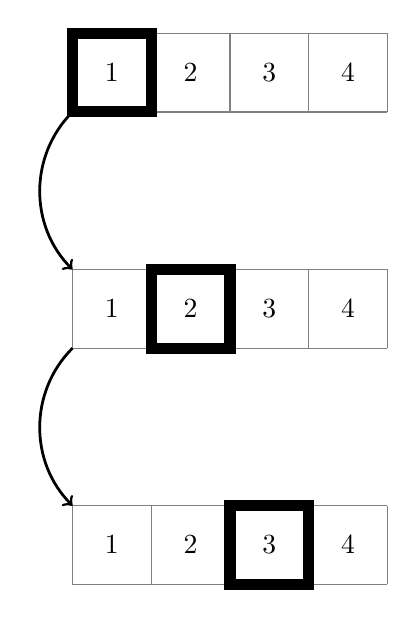
\begin{tikzpicture}[
	box/.style={rectangle,draw=black,thick, minimum size=1cm},
]
	\draw[step=1cm,color=gray] (0,0) grid (4,1);
	\node at (0.5,0.5) {1};
	\node at (1.5,0.5) {2};
	\node at (2.5,0.5) {3};
	\node at (3.5,0.5) {4};
	\draw[color=black,line width=4pt] (0,0) rectangle (1,1);

	\draw[step=1cm,color=gray] (0,-2) grid (4,-3);
	\node at (0.5,-2.5) {1};
	\node at (1.5,-2.5) {2};
	\node at (2.5,-2.5) {3};
	\node at (3.5,-2.5) {4};
	\draw[color=black,line width=4pt] (1,-2) rectangle (2,-3);

	\draw[step=1cm,color=gray] (0,-5) grid (4,-6);
	\node at (0.5,-5.5) {1};
	\node at (1.5,-5.5) {2};
	\node at (2.5,-5.5) {3};
	\node at (3.5,-5.5) {4};
	\draw[color=black,line width=4pt] (2,-5) rectangle (3,-6);

	\draw[->,line width=1pt] (0,0) to [out=-135,in=135] (0,-2);
	\draw[->,line width=1pt] (0,-3) to [out=-135,in=135] (0,-5);
\end{tikzpicture}
\end{center}
\end{column}

\begin{column}{0.48\textwidth}
\textbf{Temporal Locality}\\
\begin{itemize}
\item Data that is referenced in the near past is likely to be accessed in the near future
\end{itemize}
\vspace{1em}
\begin{center}
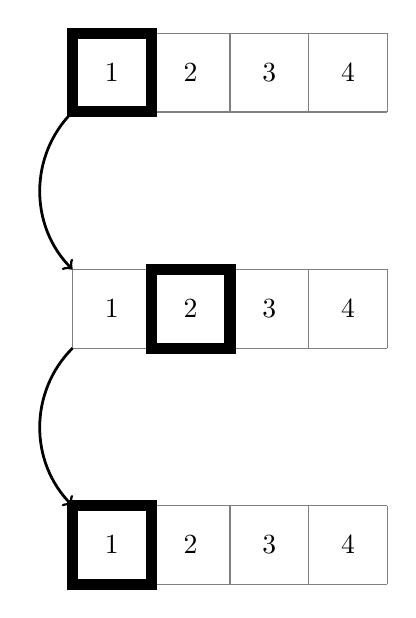
\begin{tikzpicture}[
	box/.style={rectangle,draw=black,thick, minimum size=1cm},
]
	\draw[step=1cm,color=gray] (0,0) grid (4,1);
	\node at (0.5,0.5) {1};
	\node at (1.5,0.5) {2};
	\node at (2.5,0.5) {3};
	\node at (3.5,0.5) {4};
	\draw[color=black,line width=4pt] (0,0) rectangle (1,1);

	\draw[step=1cm,color=gray] (0,-2) grid (4,-3);
	\node at (0.5,-2.5) {1};
	\node at (1.5,-2.5) {2};
	\node at (2.5,-2.5) {3};
	\node at (3.5,-2.5) {4};
	\draw[color=black,line width=4pt] (1,-2) rectangle (2,-3);

	\draw[step=1cm,color=gray] (0,-5) grid (4,-6);
	\node at (0.5,-5.5) {1};
	\node at (1.5,-5.5) {2};
	\node at (2.5,-5.5) {3};
	\node at (3.5,-5.5) {4};
	\draw[color=black,line width=4pt] (0,-5) rectangle (1,-6);

	\draw[->,line width=1pt] (0,0) to [out=-135,in=135] (0,-2);
	\draw[->,line width=1pt] (0,-3) to [out=-135,in=135] (0,-5);
\end{tikzpicture}
\end{center}
\end{column}
\end{columns}
\end{frame}


\subsection{Processor-Memory Performance Gap}

\begin{frame}{Memory-Related Performance Problems | Processor-Memory Performance Gap}
\begin{center}
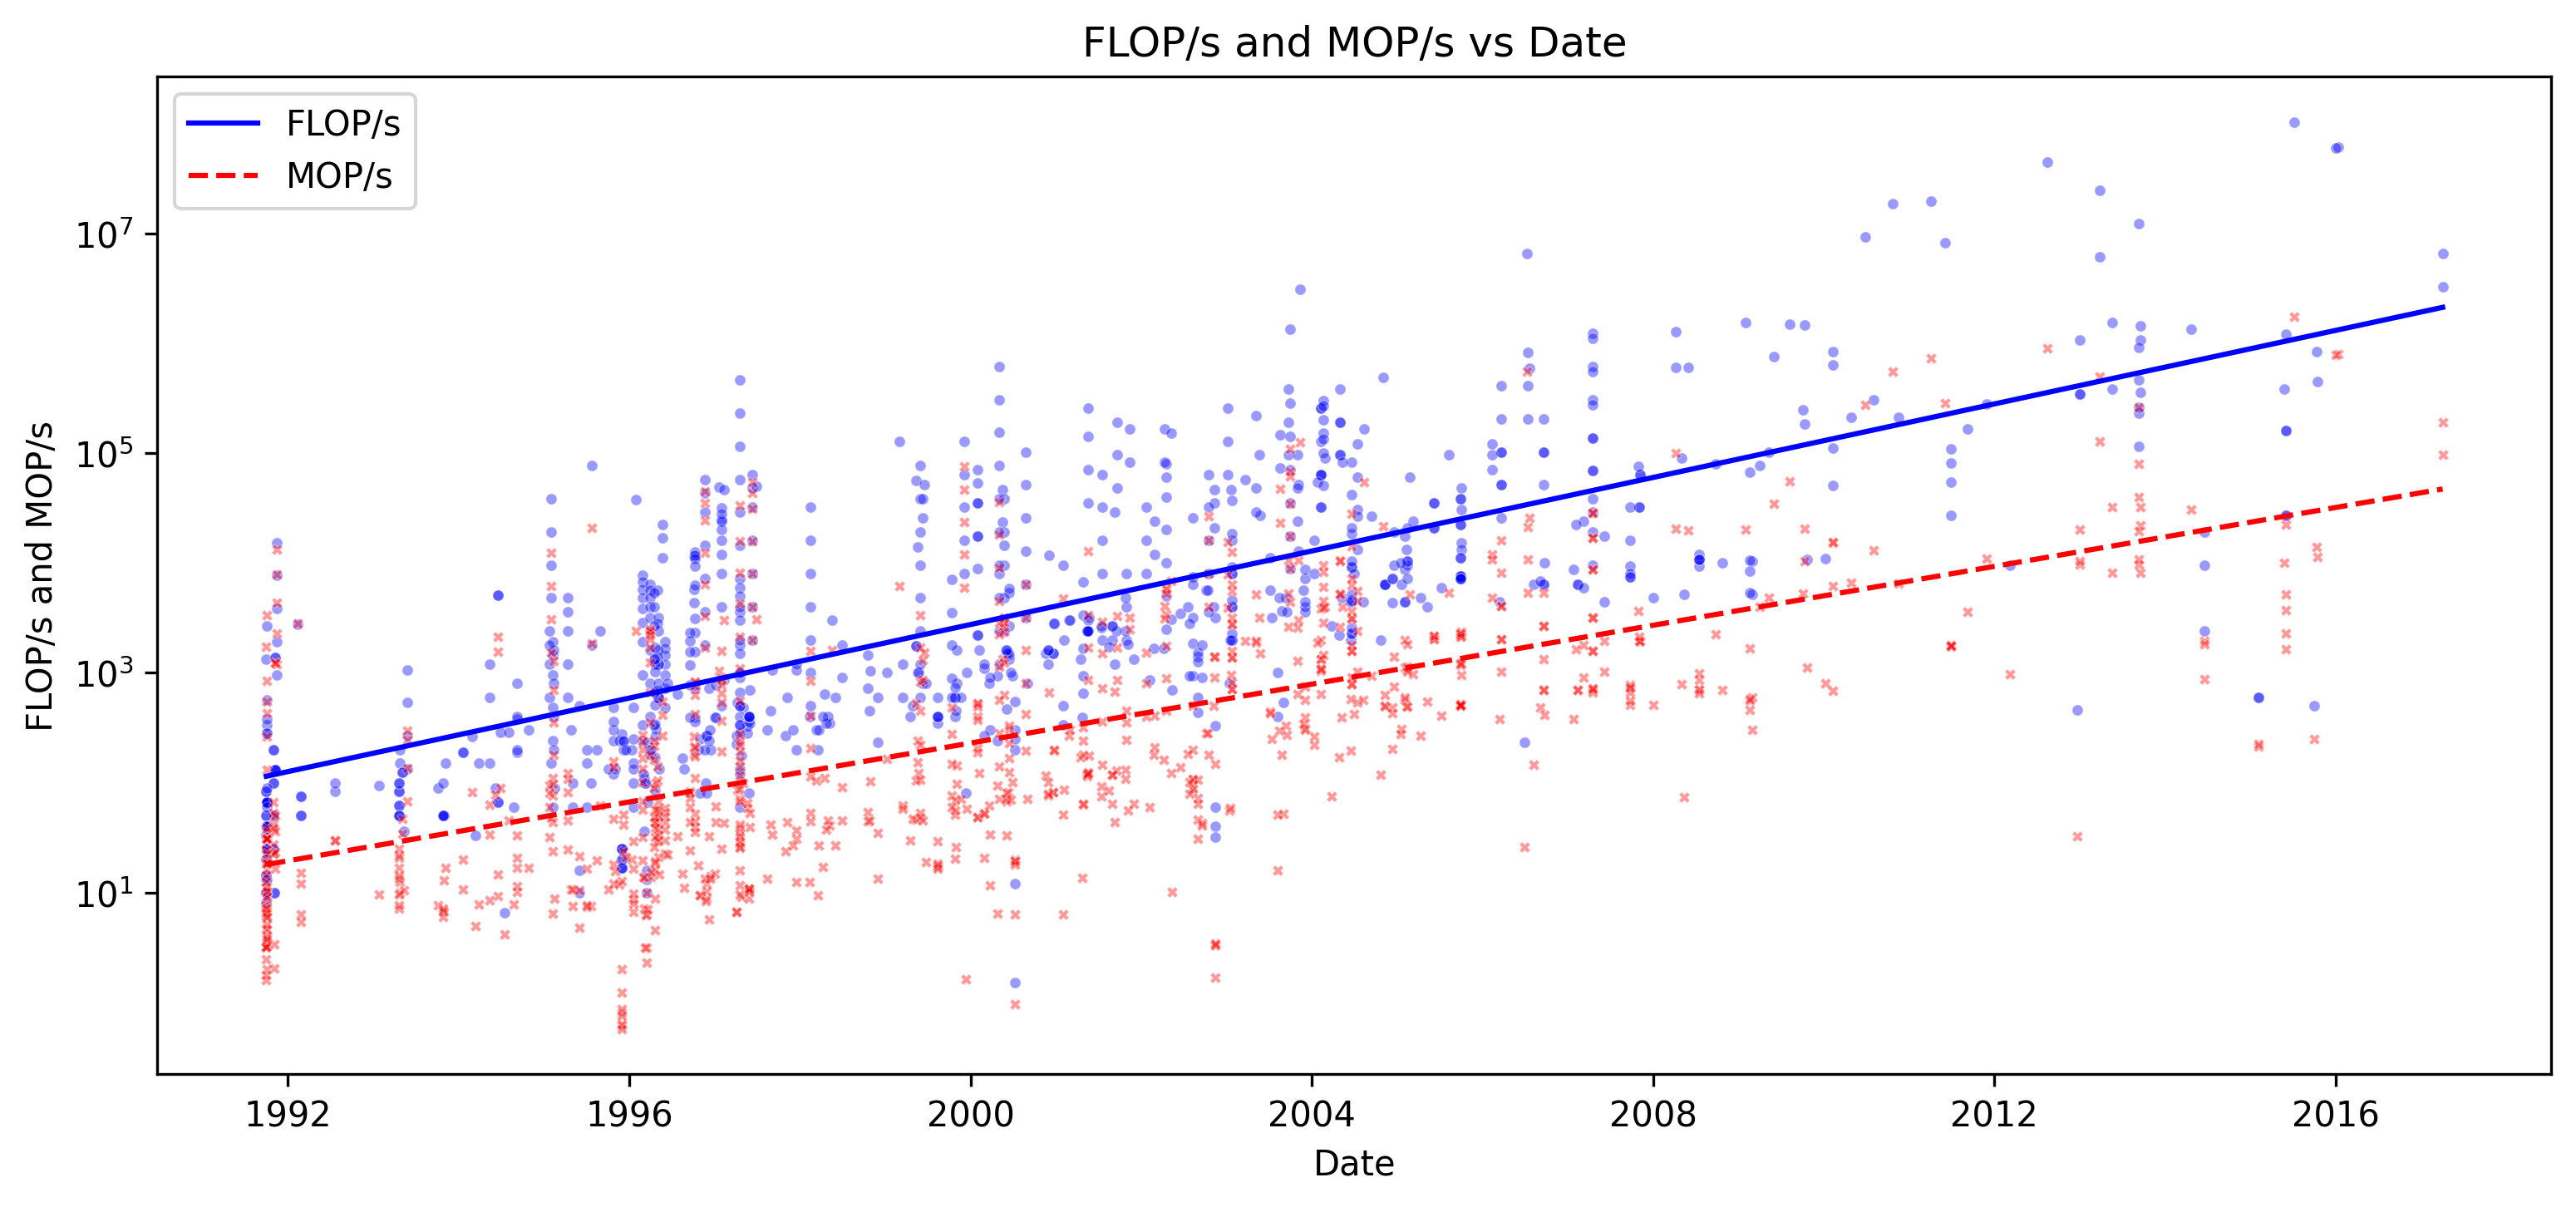
\includegraphics[height=0.8\textheight]{logos/FLOPs_MOPs_vs_Date.png}
\end{center}
\end{frame}

\section{Overview of the Optimization Workflow}
\begin{frame}[label=overview]{Overview of the Optimization Workflow}{Visualization-Guided Optimization}
\begin{center}
\smartdiagramset{
	font=\fontsize{20pt}{20pt}\selectfont,
	uniform color list=blue!40 for 3 items,
	circular distance=4cm,
	arrow tip=to,
	arrow line width=2pt,
	module minimum width=6cm,
	module minimum height=2cm,
	text width=6cm,
	additions={
		additional item font=\fontsize{20pt}{20pt}\selectfont,
		additional item bottom color=blue!40,
		additional item border color=gray,
		additional item shadow=drop shadow,
		additional item offset=3cm,
		additional item width=6cm,
		additional item height=2cm,
		additional item text width=6cm,
		additional arrow line width=2pt,
		additional arrow tip=to,
		additional arrow color=blue!40,
	}
}
\smartdiagramadd[circular diagram]{
Program,
Data Gathering,
Visualization\\Recommendations
}{right of module3/Optimized Program,left of module1/Original Program}
\smartdiagramconnect{-to}{module3/additional-module1}
\smartdiagramconnect{to-}{module1/additional-module2}
\end{center}
\end{frame}

\section{Data Gathering Approaches}
\begin{frame}{Data Gathering Approaches}{Goal: Acquire Memory-Related Data for Visualization}
\begin{itemize}
	\item Data Accesses
	\begin{itemize}
		\item Memory locations / variables
		\item Frequencies
	\end{itemize}
	\item Data access patterns
	\begin{itemize}
		\item Nested loops
	\end{itemize}
	\item Cache performance
	\begin{itemize}
		\item Hit/miss rates
		\item Utilization
		\item Amount of data transfer in between different cache levels and main memory
	\end{itemize}
\end{itemize}
\end{frame}

\begin{frame}{Data Gathering Approaches | Dynamic Analyis}{Run Program and Capture Memory-Related Information}
\begin{itemize}
	\item Hardware counters
	\begin{itemize}
		\item Counts cache hits/misses
	\end{itemize}
	\item Tracing / profiling
	\item Store source code references alongside memory-related information
\end{itemize}
\begin{columns}
\begin{column}{0.48\textwidth}
{
\setbeamertemplate{itemize item}{\color{ForestGreen} \large \faSmileO }
\begin{itemize}
	\item Very accurate
	\begin{itemize}
		\item Real program data
		\item Actual physical hardware
	\end{itemize}
\end{itemize}
}
\end{column}
\begin{column}{0.48\textwidth}
{
\setbeamertemplate{itemize item}{\color{OrangeRed} \large \faFrownO }
\begin{itemize}
	\item Can be very slow
	\item Possible large overhead for very granular data
	\item Cannot easily analyze just parts of the program
\end{itemize}
}
\end{column}
\end{columns}
\end{frame}

\begin{frame}{Data Gathering Approaches | Static Analyis}{Analyze the Programs Source Code for Data Accesses}
\begin{columns}[T]
\begin{column}{0.48\textwidth}
\begin{itemize}
	\item Extract any data access information purely from the source code
	\item Compile the program into a Data-Flow Oriented IR
	\item Statistics gathered by analyzing the IR
	\begin{itemize}
		\item Algorithmic intensity
		\item Volume of data circulating in the program
	\end{itemize}
\end{itemize}
\end{column}
\begin{column}{0.51\textwidth}
\centering
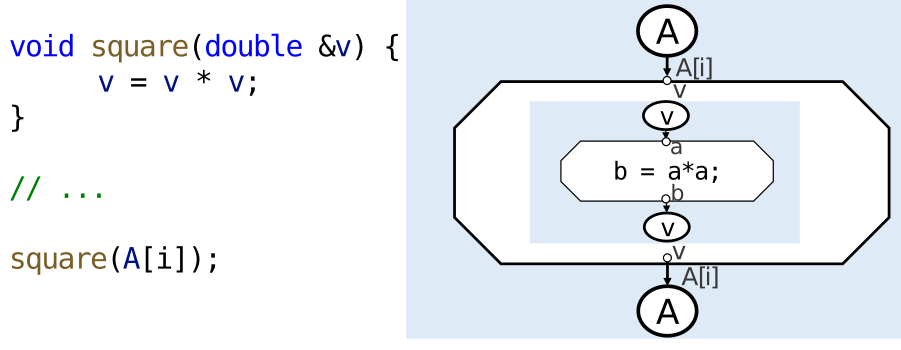
\includegraphics[width=\textwidth]{logos/SDFG.png}
\parbox{\textwidth}{\hspace*{15pt}\scriptsize Source:\thinspace{\small\itshape Alexandru Calotoiu et al. “Lifting C semantics for dataflow optimization”. In: Proceedings of the 36th ACM International Conference on Supercomputing. 2022, pp. 1-13.}}
\end{column}
\end{columns}
\end{frame}


\begin{frame}{Data Gathering Approaches | Static Analyis}{Analyze the Programs Source Code for Data Accesses}
\begin{columns}[T]
\begin{column}{0.43\textwidth}
\centering
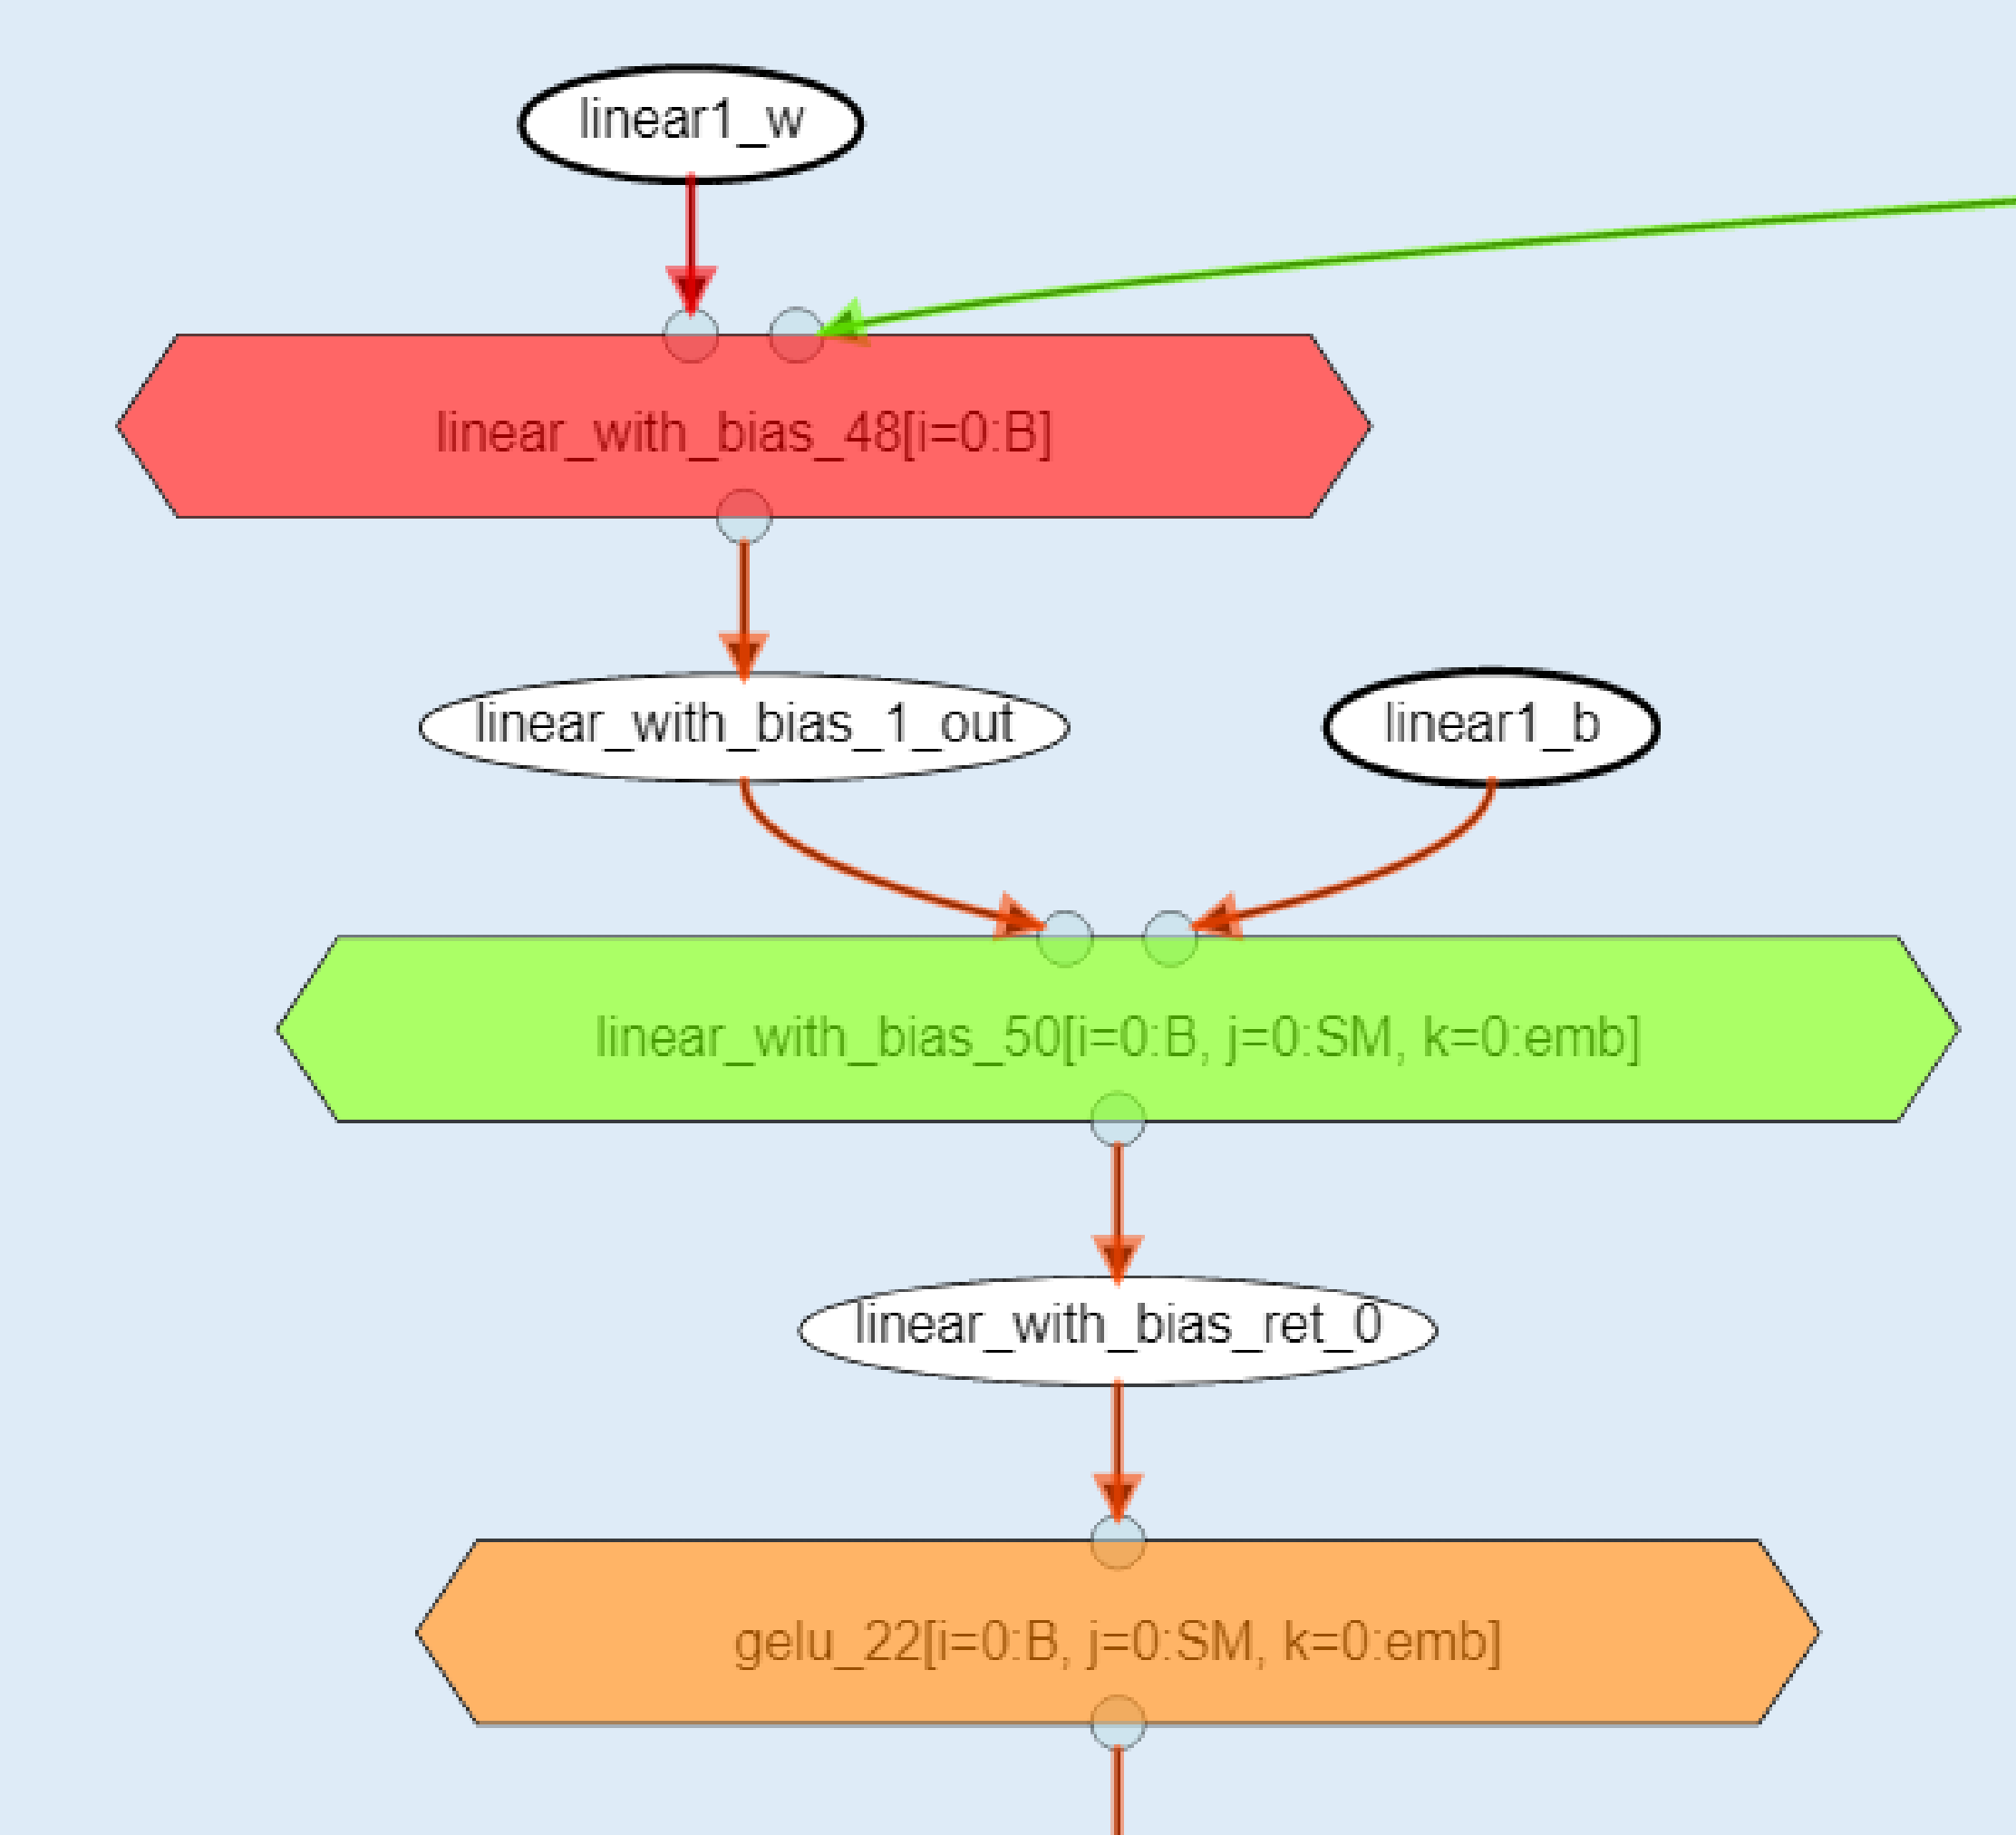
\includegraphics[height=0.6\textheight]{logos/small.png}
\parbox{\textwidth}{\hspace*{15pt}\scriptsize Source:\thinspace{\small\itshape Alexandru Calotoiu et al. “Lifting C semantics for dataflow optimization”. In: Proceedings of the 36th ACM International Conference on Supercomputing. 2022, pp. 1-13.}}
\end{column}
\begin{column}{0.53\textwidth}
{
\setbeamertemplate{itemize item}{\color{ForestGreen} \large \faSmileO }
\begin{itemize}
	\item Very fast
	\item Provides holistic view of the program and its performance
\end{itemize}
}
\vspace*{2em}
{
\setbeamertemplate{itemize item}{\color{OrangeRed} \large \faFrownO }
\begin{itemize}
	\item Very abstract analysis
	\begin{itemize}
		\item Memory layout of data is not considered
		\item Hardware architecture unknown
		\item No information about real-world cache performance
	\end{itemize}
\end{itemize}
}
\end{column}
\end{columns}
\end{frame}


\begin{frame}{Data Gathering Approaches | Cache Simulation}{Imitate the Programs Memory Accesses on a Simulated Cache Hierarchy}
\begin{itemize}
	\item Replicate actual hardware through software
	\begin{itemize}
		\item Cache hierarchy (size, associativity, etc.)
		\item Cache replacement policies
		\item Cache coherence protocols
	\end{itemize}
	\item Simulate the programs memory-wise on the simulated hardware
	\begin{itemize}
		\item Memory (de-)allocations
		\item Data accesses
	\end{itemize}
\end{itemize}
\begin{columns}
\begin{column}{0.48\textwidth}
{
\setbeamertemplate{itemize item}{\color{ForestGreen} \large \faSmileO }
\begin{itemize}
	\item Very detailed
	\begin{itemize}
		\item Insights about the memory-layout of data
		\item Enables step-by-step analysis of the caches
	\end{itemize}
	\item Allows to analyze only parts of the program
\end{itemize}
}
\end{column}
\begin{column}{0.48\textwidth}
{
\setbeamertemplate{itemize item}{\color{OrangeRed} \large \faFrownO }
\begin{itemize}
	\item Requires precise parameterization
\end{itemize}
}
\end{column}
\end{columns}
\end{frame}

\section{Visualization Techniques}

\begin{frame}{Visualization Techniques}{Goal: Display Bottlenecks (and explain them)}

\end{frame}

\againframe{overview}

\section{Specific Optimization Tool}

\section{Conclusion}

\begin{frame}[allowframebreaks]{References}
\begin{itemize}
\item[\faBook] Alexandru Calotoiu et al. “Lifting C semantics for dataflow optimization”. In: \textit{Proceedings of the 36th ACM International Conference on Supercomputing}. 2022, pp. 1-13.
\end{itemize}
\end{frame}

\end{document}
